\documentclass{article}
\usepackage{amsmath}
\usepackage{tcolorbox}
\usepackage{graphicx}

\begin{document}

\title{7.2 Trigonometric Integrals}
\author{GitHub Copilot}
\date{\today}

\maketitle

\section{Introduction}

Trigonometric integrals are integrals that involve trigonometric functions. They often require techniques such as substitution, trigonometric identities, or integration by parts to solve.

\section{Basic Trigonometric Integrals}

The basic trigonometric integrals are:

\begin{align*}
    \int \sin(x) \, dx &= -\cos(x) + C \\
    \int \cos(x) \, dx &= \sin(x) + C \\
    \int \tan(x) \, dx &= -\ln|\cos(x)| + C \\
    \int \cot(x) \, dx &= \ln|\sin(x)| + C \\
    \int \sec(x) \, dx &= \ln|\sec(x) + \tan(x)| + C \\
    \int \csc(x) \, dx &= -\ln|\csc(x) + \cot(x)| + C
\end{align*}

\section{Strategies for Solving Trigonometric Integrals}

When faced with a trigonometric integral, there are several strategies that can be used:

1. **Use a Pythagorean identity**: This can simplify the integral and make it easier to solve.
2. **Use a double-angle formula**: This can reduce the power of the trigonometric function.
3. **Use a half-angle formula**: This can also reduce the power of the trigonometric function.
4. **Use substitution**: This can simplify the integral and make it easier to solve.
5. **Use integration by parts**: This can be used when the integral is the product of two functions.

In the following sections, we will look at examples that demonstrate these strategies.

\section{Example 1}

Let's look at an example. Suppose we want to integrate $\int \cos^3(x) \, dx$.

For this integral, we can use the power-reducing identity $\cos^2(x) = 1 - \sin^2(x)$ to rewrite the integral as:

\begin{align*}
    \int \cos^3(x) \, dx &= \int \cos(x) \cdot \cos^2(x) \, dx \\
    &= \int \cos(x) \cdot (1 - \sin^2(x)) \, dx
\end{align*}

Now we can use substitution with $u = \sin(x)$ and $du = \cos(x) \, dx$:

\begin{align*}
    \int \cos(x) \cdot (1 - \sin^2(x)) \, dx &= \int (1 - u^2) \, du \\
    &= u - \frac{1}{3} u^3 + C \\
    &= \sin(x) - \frac{1}{3} \sin^3(x) + C
\end{align*}

So, $\int \cos^3(x) \, dx = \sin(x) - \frac{1}{3} \sin^3(x) + C$.

\section{Example 2}

Let's look at another example. Suppose we want to integrate $\int_0^\pi \sin^2(x) \, dx$.

For this integral, we can use the power-reducing identity $\sin^2(x) = \frac{1 - \cos(2x)}{2}$ to rewrite the integral as:

\begin{align*}
    \int_0^\pi \sin^2(x) \, dx &= \int_0^\pi \frac{1 - \cos(2x)}{2} \, dx \\
    &= \frac{1}{2} \int_0^\pi dx - \frac{1}{2} \int_0^\pi \cos(2x) \, dx
\end{align*}

The first integral is straightforward, and the second integral can be solved by using the basic integral of cosine:

\begin{align*}
    \frac{1}{2} \int_0^\pi dx - \frac{1}{2} \int_0^\pi \cos(2x) \, dx &= \frac{1}{2} [x]_0^\pi - \frac{1}{2} [\frac{1}{2} \sin(2x)]_0^\pi \\
    &= \frac{\pi}{2} - 0 \\
    &= \frac{\pi}{2}
\end{align*}

So, $\int_0^\pi \sin^2(x) \, dx = \frac{\pi}{2}$.

\section{Example 3}

Let's look at another example. Suppose we want to integrate $\int \sin^4(x) \, dx$.

For this integral, we can use the half-angle formula $\sin^2(x) = \frac{1 - \cos(2x)}{2}$ to rewrite the integral as:

\begin{align*}
    \int \sin^4(x) \, dx &= \int \left(\frac{1 - \cos(2x)}{2}\right)^2 \, dx \\
    &= \frac{1}{4} \int (1 - 2\cos(2x) + \cos^2(2x)) \, dx
\end{align*}

Now we can use the half-angle formula again to rewrite $\cos^2(2x)$ as $\frac{1 + \cos(4x)}{2}$:

\begin{align*}
    \frac{1}{4} \int (1 - 2\cos(2x) + \cos^2(2x)) \, dx &= \frac{1}{4} \int (1 - 2\cos(2x) + \frac{1 + \cos(4x)}{2}) \, dx \\
    &= \frac{1}{4} \int (1 - 2\cos(2x) + \frac{1}{2} + \frac{1}{2}\cos(4x)) \, dx \\
    &= \frac{1}{4} \int \left(\frac{3}{2} - 2\cos(2x) + \frac{1}{2}\cos(4x)\right) \, dx
\end{align*}

The integral can now be solved by using the basic integrals of cosine:

\begin{align*}
    \frac{1}{4} \int \left(\frac{3}{2} - 2\cos(2x) + \frac{1}{2}\cos(4x)\right) \, dx &= \frac{1}{4} \left[\frac{3}{2}x - \sin(2x) + \frac{1}{8}\sin(4x)\right] + C \\
    &= \frac{3}{8}x - \frac{1}{4}\sin(2x) + \frac{1}{32}\sin(4x) + C
\end{align*}

So, $\int \sin^4(x) \, dx = \frac{3}{8}x - \frac{1}{4}\sin(2x) + \frac{1}{32}\sin(4x) + C$.

\begin{figure}[h]
    \centering
    
\includegraphics[width=1\textwidth]{../assets/image.png}
    \caption{}
    \label{fig:my_label}
\end{figure}
\begin{figure}[h]
    \centering
    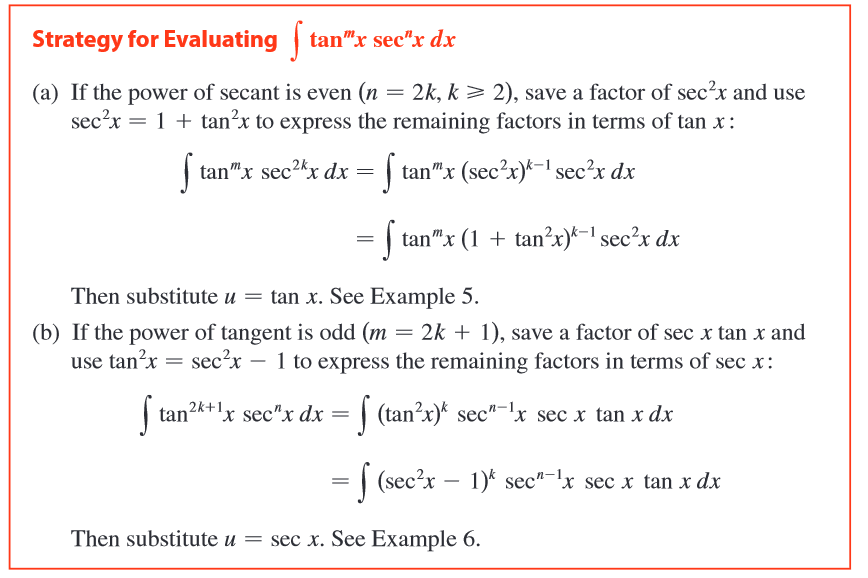
\includegraphics[width=1\textwidth]{../assets/image2.png}
    \caption{}
    \label{fig:squidward}
\end{figure}

\begin{figure}[h]
    \centering
    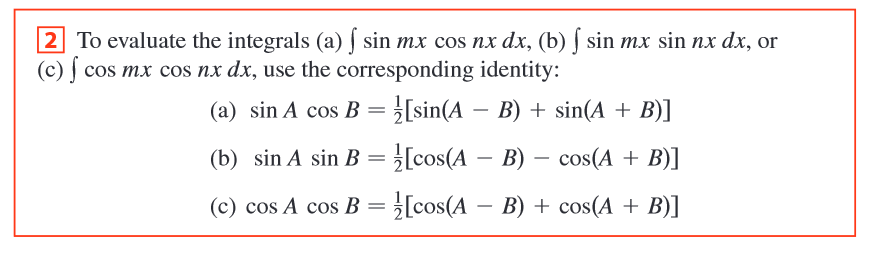
\includegraphics[width=1\textwidth]{../assets/image3.png}
    \caption{}
    \label{fig:squidwardv2}
\end{figure}


\end{document}